В Казахстане есть $N$ городов, пронумерованных целыми числами от 0 до $N - 1$. Кроме того, в
стране есть неизвестное количество мегаполисов. И город и мегаполис, без уточнения какой
именно, называются \textit{населенными пунктами}.

Все населенные пункты в Казахстане соединены единой сетью двусторонних дорог. Каждая
дорога соединяет два различных населенных пункта. Каждая пара населенных пунктов
напрямую соединена не более, чем одной дорогой. Для любой пары населенных пунктов $a$ и $b$
существует единственный способ добраться по дорогам от одного населенного пункта до
другого, не использующий ни одну дорогу более одного раза.

Известно, что город всегда соединен дорогой напрямую ровно с одним населенным пунктом, а
мегаполис~--- хотя бы с тремя населенными пунктами.

На иллюстрации ниже показана сеть дорог, состоящая из 11 городов и 7 мегаполисов. Города
обозначены кругами с числами, а мегаполисы~--- квадратами с буквами.

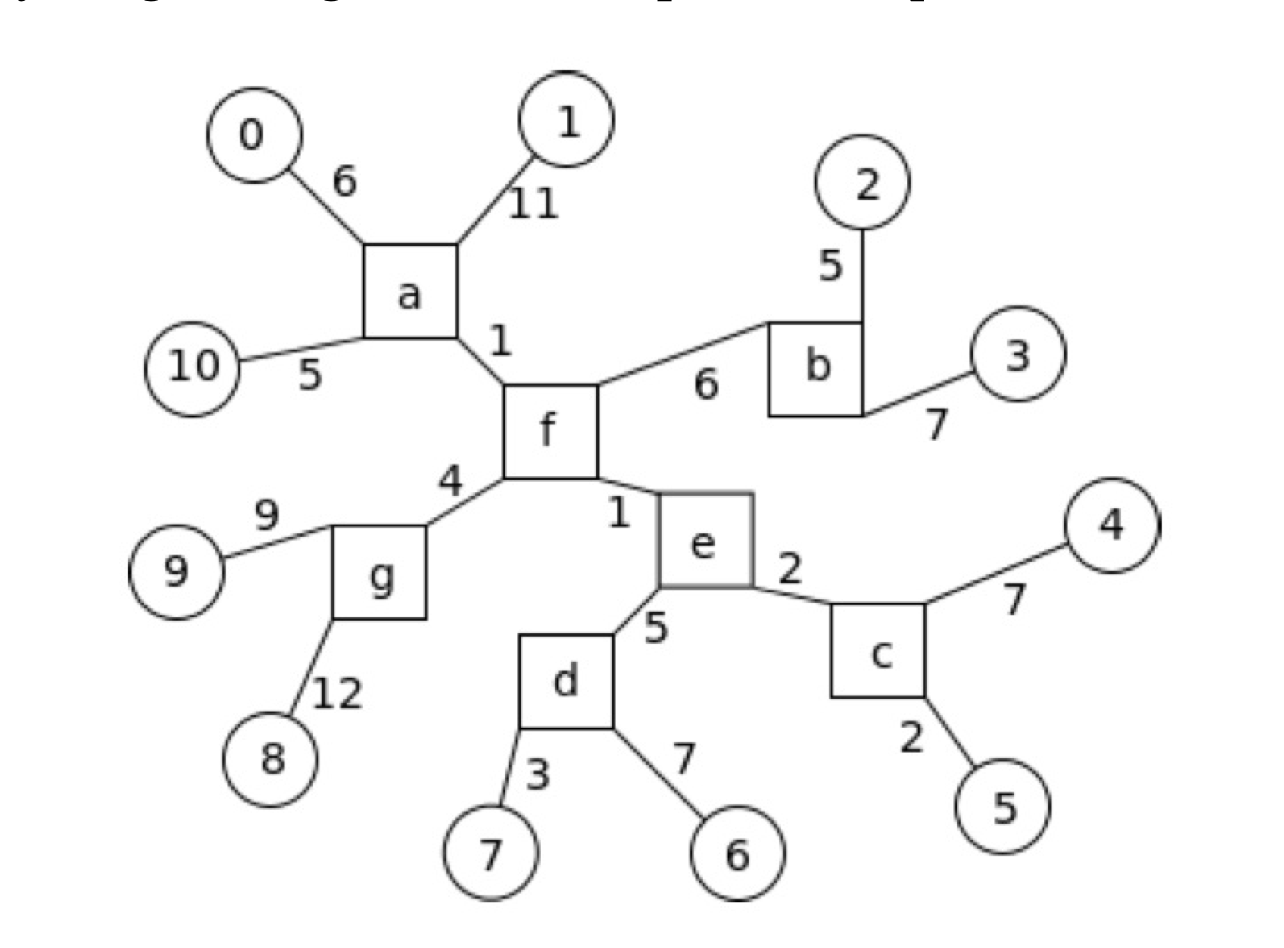
\includegraphics[scale=0.8]{towns.png}

Длина каждой дороги~--- это положительное целое число. Расстояние между двумя
населенными пунктами определяется как минимальная сумма длин дорог, которые
необходимо проехать, чтобы добраться из одного города в другой.

Для каждого мегаполиса $C$ можно определить расстояние до города, который расположен
дальше всего. Обозначим это расстояние $r(C)$. Будем называть мегаполис $C$ транспортным
узлом, если расстояние $r(C)$ минимально среди всех мегаполисов. Расстояние между
транспортным узлом и самым далеким от него городом обозначим $R$. Таким образом, $R$~---
это минимальное из значений $r(C)$.

На примере выше самый далекий город от мегаполиса $a$~--- восьмой, а расстояние между
ними равно 17 $(r(a) = 1 + 4 + 12)$. Для мегаполиса $g$ расстояние $r(g)$ также равно 17.
Самый далекий город от него~--- шестой. Единственный транспортный узел в этом примере~---
это мегаполис $f$, для которого расстояние $r(f) = 16$. Таким образом, $R = 16$.

При удалении любого транспортного узла сеть дорог распадается на несколько связных
частей. Транспортный узел называется \textit{сбалансированным}, если в каждой из таких частей
находится не более $\lfloor \frac{N}{2} \rfloor$ городов. Обратите внимание, что мегаполисы не учитываются.
Обозначение $\lfloor x \rfloor$ означает максимальное целое число, не превосходящее $x$.

В примере мегаполис $f$ является транспортным узлом. При его удалении сеть дорог
распадется на четыре связные части. Эти четыре части содержат следующие города:
{$0,1,10$}, {$2,3$}, {$4,5,6,7$} и {$8,9$}. Ни в одной из этих частей нет более пяти городов
($\lfloor \frac{11}{2} \rfloor = 5$), поэтому мегаполис $f$~--- это сбалансированный транспортный узел.

\textbf{Постановка задачи}

Изначально о системе дорог ничего не известно, кроме числа $N$~--- количества городов. Не
известно число мегаполисов, а также ничего не известно о расположении дорог в стране.
Можно получать информацию о сети дорог с помощью запросов расстояния между парами
городов.

Необходимо определить:
\begin{itemize}
\item Во всех подзадачах: расстояние $R$.
\item В подзадачах с $3$ по $6$: есть ли в сети дорог сбалансированный транспортный узел.
\end{itemize}

Необходимо реализовать функцию \texttt{hubDistance}. В каждом тесте может быть несколько
наборов входных данных. Количество наборов входных данных в одном тесте не превосходит
40. Для каждого набора входных данных функция \texttt{hubDistance} будет вызвана ровно один раз.
Убедитесь, что все необходимые переменные инициализируются каждый раз, когда
вызывается эта функция.

\begin{itemize}
\item \texttt{int hubDistance(int N, int sub)}
\begin{itemize} 
\item $N$~--- количество городов.
\item $sub$~--- номер подзадачи (см. подзадачи).
\item Если $sub$ равно 1 или 2, функция может вернуть $R$ или $-R$.
\item Если $sub$ больше 2, то, если существует сбалансированный транспортный узел,
функция должна вернуть $R$, иначе она должна вернуть $-R$.
\end{itemize}
\end{itemize}

Функция \texttt{hubDistance} может получить информацию о системе дорог, используя функцию
\texttt{getDistance(i, j)}. Эта функция возвращает расстояние между городами $i$ и $j$. Если $i$ и $j$
равны, функция возвращает $0$. Если функции передать некорректные аргументы, то она также
возвращает $0$.



